\documentclass{jknotes}
\usepackage{../joshkirklin}

\setmathfont{Latin Modern Math}
\setmathfont{GFS NeoHellenic Math}[range=bfsfup/{greek,Greek}->it]
\setmathfont{GFS NeoHellenic Math}[range=sfup/{latin,Latin}->it]

\usetikzlibrary{shapes.misc, pgfplots.fillbetween}
\renewcommand{\u}{\symbf{u}}
\newcommand{\Ra}{\text{Ra}}

\tikzset{cross/.style={cross out, draw=black, minimum
size=2*(#1-\pgflinewidth), inner sep=0pt, outer sep=0pt}}
%default radius will be 1pt. 

\newcommand{\myol}[2][3]{{}\mkern#1mu\overline{\mkern-#1mu#2}}

\begin{document}

\institution{Cambridge Part III Maths}
\title{Hydrodynamic Stability}
\lecturer{Prof. Richard Kerswell}
\notetaker{Charles Powell}
\date{Lent 2020}

\maketitle
\suggestionsspiel
\tableofcontents

\section{Introduction}
We are typically interested in whether a given flow solution $\u(\x,t)$ is
`stable', certainly to small (infinitesimal) disturbances and perhaps to
larger perturbations too. We perturb $\u(\x)$ to $\u(\x) + \hat{\u}(\x,t)$ and
define the \emph{perturbation energy} as
\begin{equation}
	E(t) \equiv \int \frac{1}{2}\hat{\u}^2(\x,t) \, \diffd V
\end{equation}
A solution is said to be stable if
\begin{equation}
	\lim_{t \to \infty} \frac{E(t)}{E(0)} = 0
\end{equation}
for all perturbations $\hat{\u}$. Conversely, if there exists $\hat{\u}$ such
that $E(t) \not\rightarrow 0$ then $\u$ is unstable. The nature of $E(0)$
determines the type of perturbation:
\begin{itemize}
	\item If $E(0) \to 0$ we have an infinitesimal disturbance
	\item If $E(0) < \delta$ then we probe finite amplitude disturbances
	\item If $E(0) \to \infty$ this probes the \emph{global} stability
\end{itemize}

In the first 9 lectures we focus on the first situation, which is linear
stability analysis. Consider the Navier-Stokes equations
\begin{align}
	\frac{\partial \u}{\partial t} + \u \cdot \nabla \u + \nabla p =
	\frac{1}{\text{Re}} \nabla^2 \u
\end{align}

If $\symbf{U}(\x)$ is a steady (basic) solution then
\begin{equation}
	\symbf{U}\cdot\nabla\symbf{U} + \nabla P = \frac{1}{\text{Re}} \nabla^2
	\symbf{U}
\end{equation}
Let $\u = \symbf{U}(\x) + \hat{\u}(\x,t), p = P + \hat{p}$. Then
\begin{equation}
	\frac{\partial \hat{\u}}{\partial t} + \u \cdot \nabla \symbf{U} +
	\symbf{U} \cdot \nabla \hat{\u} + \cancel{\hat{\u}\cdot\nabla\hat{\u}} +
	\nabla \hat{p} = \frac{1}{\text{Re}} \nabla^2 \hat{\u}
\end{equation}
The term $\hat{u}\cdot\nabla \symbf{U}$ is stabilising whilst the term
$\nabla^2 \hat{u} / \text{Re}$ is destabilising. Therefore, we expect stability
as $\text{Re} \to 0$ the stabilising term dominates, and instability as
$\text{Re} \to \infty$ when the destablising term dominates. Thus there exists
some value $\text{Re}_{\text{crit}}$ at which instability arises. We will ask
what this value is, and what is the form of the initial
instability/mode/pattern?

\section{Kelvin-Helmholtz instability}
See Drazin (2002), section 3.3, pages 47--50. Here we take a different approach
and derive Rayleigh's equation (example 8.3, page 151 of Drazin). 

\begin{center}
	\begin{tikzpicture}
		\draw[thick,->] (-3, 0) -- (3, 0) node[right] {$x$};
		\draw[dashed,->] (0, -1.5) -- (0, 1.5) node[above] {$z$};
		\draw[blue,dashed] (1.5, 0) -- (1.5, 1.4);
		\draw (1.5, 0) node[below] {$U$};
		\draw (-1.5, 0) node[above] {$-U$};
		\draw[blue,dashed] (-1.5, 0) -- (-1.5, -1.4);

		\draw[blue,->] (0, 0.4) -- (1.5, 0.4);
		\draw[blue,->] (0, 0.8) -- (1.5, 0.8);
		\draw[blue,->] (0, 1.2) -- (1.5, 1.2);
		\draw[blue,->] (0, -0.4) -- (-1.5, -0.4);
		\draw[blue,->] (0, -0.8) -- (-1.5, -0.8);
		\draw[blue,->] (0, -1.2) -- (-1.5, -1.2);
	\end{tikzpicture}
\end{center}

Consider a flow $\u = U(z)\hat{\x}$ where
\begin{equation}
	U(z) = \begin{cases} U & z > 0 \\ -U & z < 0 \end{cases}
\end{equation}
The linearised, \emph{inviscid} equation for perturbation $\hat{\u}$ is
\begin{align}
	\frac{\partial \hat{\u}}{\partial t} + \hat{w}U'\hat{\x} + U
	\frac{\partial \hat{\u}}{\partial x} + \nabla \hat{p} &= 0 \\
	\nabla \cdot \hat{\u} &= 0 
\end{align}
The boundary conditions are $\hat{\u} \to 0$ as $z \to \pm \infty$, i.e. no
energy is radiated in from infinity. We will work in 2D with velocity
components $(\hat{u},\hat{w}) = (\psi_z, -\psi_x)$ and let $\psi(x,z,t) =
\phi(z) e^{i\alpha(x-ct)}$ where $c$ is a complex eigenvalue, currently
unknown. Formally, this is equivalent to taking a Fourier transform. We have
\begin{equation}
	i\alpha (U-c) \begin{pmatrix} \phi' \\ -i\alpha \phi \end{pmatrix} +
	\begin{pmatrix} -i\alpha U' \phi \\ 0 \end{pmatrix} + \begin{pmatrix} i
\alpha p \\ \frac{\partial p}{\partial z} \end{pmatrix} = 0
\end{equation}
We can eliminate $p$ via $\partial_z (\text{top}) - i\alpha(\text{bottom})$ to
get
\begin{equation}
	(U-c)(\phi''-\alpha^2 \phi) - U'' \phi = 0
\end{equation}
with boundary conditions $\phi \to 0$ as $z \to \pm \infty$. This is
\emph{Rayleigh's equation}. Note that $c$ is the crucial eigenvalue. We wish to
know when $c_i = \Im(c) > 0$ as a function of $U(z)$, as $c_i$ is the growth
rate:
\begin{equation}
	\hat{u} \propto e^{i\alpha(x-ct)} = e^{i\alpha(c-c_r t - i c_i t)} =
		e^{i\alpha(x-c_r t) + \alpha c_i t}
\end{equation}
Note the following:
\begin{itemize}
	\item There is a symmetry $\alpha \mapsto -\alpha$, so without loss of
		generality we consider $\alpha > 0$.
	\item The complex conjugate is also a solution with $c \mapsto c^*$. Hence
		an unstable mode has a damped partner, so we have stability only if
		all modes are `neutral' i.e. $c_i = 0$. 
	\item There is a possible singularity at $y$ where $U(y) = c$, called the
		\emph{critical layer}. If $c$ is real, see later.
\end{itemize}

We now solve Rayleigh's equation with $U(z)$ defined as before. We solve above
and below $z=0$ and piece the solutions together. Since $U'' = 0$, we have
\begin{equation}
	\phi'' = \alpha^2 \phi
\end{equation}
which admits a solution satisfying the boundary conditions:
\begin{equation}
	\phi = \begin{cases} A^{-\alpha z} & z > 0 \\ B e^{\alpha z} & z < 0 
	\end{cases}
\end{equation}

The matching conditions at $z=0$ are
\begin{enumerate}
	\item Pressure $\hat{p}$ continuous at $z=0$, with $\hat{p}$ given by:
		\begin{equation}
			\hat{p} = U' \phi - (U-c) \phi'
		\end{equation}
	\item Kinematic condition at the surface:
		\begin{equation}
			\frac{\diffD}{\diffD t} \left( z - \zeta(x,t)\right) = 0
		\end{equation}
		where $z=\zeta(x,t)$ is the position of the surface.
		After linearising, we have
		\begin{equation}
			 w - \frac{\partial \zeta}{\partial t} - U\frac{\partial
			 \zeta}{\partial x} = 0
		\end{equation}
	 	Inserting the form of $w$ and $U$ we require that
	 	\begin{equation}
		 	\zeta = - \frac{\phi}{U-c}
	 	\end{equation}
	 	is continuous across $z=0$.
\end{enumerate}
Requiring $p$ continuous gives
\begin{equation}
	-(U-c)A(-\alpha) = - (-U-c)B(\alpha)
\end{equation}
Requiring $\zeta$ continuous gives
\begin{equation}
	\frac{A}{U-c} = \frac{B}{-U-c}
\end{equation}
Hence we have
\begin{equation}
	(U-c)^2 = -(U+c)^2
\end{equation}
i.e. $c = \pm i U$ so the growth rate is $\alpha U$. Thus the flow is unstable
to waves of all wavelengths. The instability may be remedied 
\begin{itemize}
	\item by adding a density stratification, which stabilises long
		wavelengths (small $\alpha$)
	\item by adding surface tension, which stabilises short wavelengths (large
		$\alpha$), e.g. Drazin page 50 equation 3.21.
\end{itemize}

\section{Thermal instabilities: Rayleigh-Bernard convection}
Consider two parallel plates separated by distance $L$ with fluid subject to
gravity and temperatue difference $\Delta T$ between the plates. The lower
plate is heated to $T_0 + \Delta T$ whilst the upper plate is fixed at
temperature $T_0$. 
\begin{center}
	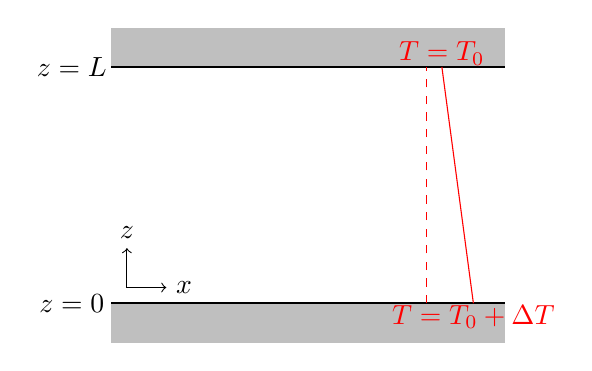
\begin{tikzpicture}
		\draw[draw=none,fill=gray!50] (0,0) rectangle (5,-0.5);
		\draw[thick] (0,0) -- (5, 0);
		\draw[draw=none,fill=gray!50] (0,3) rectangle (5,3.5);
		\draw[thick] (0,3) -- (5, 3);

		\draw[->] (0.2, 0.2) -- (0.7, 0.2) node[right] {$x$};
		\draw[->] (0.2, 0.2) -- (0.2, 0.7) node[above] {$z$};
		\draw (-0.5, 0) node {$z=0$};
		\draw (-0.5, 3) node {$z=L$};
		\draw[red,dashed] (4, 0) -- (4, 3);
		\draw[red] (4.2, 3) -- (4.6, 0);
		\draw[red] (4.2, 2.9) node[above] {$T=T_0$};
		\draw[red] (4.6, 0.1) node[below] {$T=T_0+\Delta T$};
	\end{tikzpicture}
\end{center}

The basic state consists of no motion, with heat transfer by conduction only.
\paragraph{Governing equations.}
The governing equations are those of momentum, mass, and (thermal) energy
conservation.
\begin{align}
	\rho \frac{\diffD \u}{\diffD t} + \nabla p &= \mu \nabla^2 \u + \rho g
	\hat{\symbf{z}} \\
	\frac{\partial T}{\partial t} + \u \cdot \nabla T &= \kappa \nabla^2 T \\
	\frac{\diffD \rho}{\diffD t} + \rho \nabla \cdot \u &= 0
\end{align}
To close the set of equations we need a relationship between $\rho$ and $T$.
Most cases of interest have $\Delta T$ and $\Delta \rho$ small, i.e. $\Delta
\rho \ll \rho_0, \Delta T \ll T_0$. Two consequences of this assumption are:
\begin{enumerate}
	\item We can Taylor expand $\rho = \rho(T)$:
		\begin{equation}
			\rho \approx \rho(T_0) \left[ 1 - \alpha(T-T_0)\right]
		\end{equation}
		where $\alpha > 0$ is the coefficient of thermal expansion, such that
		$T$ increases when $\rho$ decreases. We write $\rho_0 = \rho(T_0)$.
	\item We can adopt a Boussinesq approximation: acknowledge density changes
		only in the buoyancy term $\rho g \hat{\symbf{z}}$. Importantly, we
		can assume the fluid is incompressible.
\end{enumerate}

Define $\theta = T - T_0$. The governing equations are now
\begin{align}
	\rho_0 \frac{\diffD \u}{\diffD t} + \nabla p &= \mu \nabla^2 \u +
	\rho_0(1-\alpha \theta)g \hat{\symbf{z}} \\
	\frac{\partial \theta}{\partial t} + \u \cdot \nabla \theta &= \kappa
	\nabla^2 \theta \\
	\nabla \cdot \u &= 0
\end{align}

The basic state is $u = 0, \theta = \Delta T (1-z/L)$ and
\begin{equation}
	\frac{\diffd p}{\diffd z} = -\rho_0 (1-\alpha \Delta T(1-z/L))g
\end{equation}

We now non-dimensionalise using scalings $t \sim L^2/\kappa, u \sim \kappa/L,
\theta \sim \Delta T$, e.g. $\theta = \Delta T \theta^*$ where $\theta^*$ is
the non-dimensionalised variable. We normalise the $\frac{\diffD \u^*}{\diffD
t^*}$ term, to get:
\begin{align}
	\frac{\diffD \u^*}{\diffD t^*} + \nabla^* p^* &= \frac{\mu}{\rho_0 \kappa}
	\nabla^{*2} \u^* + \frac{\alpha g \Delta T L^3}{\kappa^2} \theta^* \hat{\symbf{z}} \\
	\frac{\partial \theta^*}{\partial t^*} + \u^* \cdot \nabla^* \theta^* &=
	\nabla^{*2} \theta^* \\
\end{align}
Define the \emph{Prandtl number} 
\begin{equation}
	\sigma \equiv \frac{\nu}{\kappa} = \frac{\mu}{\rho_0 \kappa}
\end{equation}
which is the ratio of viscous/momentum diffusion to thermal diffusion. Typical values
are $0.72$ in air, $7$ in water, $10^5$ in magma. We also define the
\emph{Rayleigh number}
\begin{equation}
	\text{Ra} \equiv \frac{\alpha \Delta T g L^3}{\kappa \nu}
\end{equation}
which is the ratio of destabilising buoyancy to stabilising diffusion.
Dropping the $^*$ notation, we have
\begin{align}
	\frac{\partial \u}{\partial t} + \u \cdot \nabla \u + \nabla p &= \sigma
	\nabla^2 \u + \sigma \text{Ra} \theta \hat{\symbf{z}} \\
	\frac{\partial \theta}{\partial t} + \u \cdot \nabla \theta &= \nabla^2
	\theta \\
	\nabla \cdot \u &= 0
\end{align}

\paragraph{Boundary conditions.}
There are three combinations of boundary condition available in this problem,
with the choice fixed wall (no slip) or stress free (free slip).
\begin{center}
	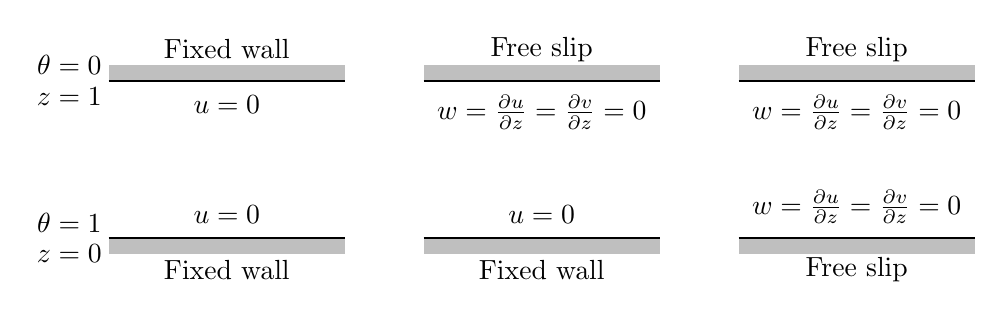
\begin{tikzpicture}
		\draw (-0.5, 0.2) node {$\theta = 1$};
		\draw (-0.5, -0.2) node {$z = 0$};
		\draw (-0.5, 2.2) node {$\theta = 0$};
		\draw (-0.5, 1.8) node {$z = 1$};

		\draw[fill=gray!50,draw=none] (0,0) rectangle (3,-0.2);
		\draw[fill=gray!50,draw=none] (0,2) rectangle (3,2.2);
		\draw[thick] (0,0) -- (3, 0);
		\draw[thick] (0,2) -- (3, 2);

		\draw (1.5, 0.3) node {$\u = 0$};
		\draw (1.5, 1.7) node {$\u = 0$};

		\draw (1.5, -0.4) node {Fixed wall};
		\draw (1.5, 2.4) node {Fixed wall};

		\begin{scope}[shift={(4, 0)}]
			\draw[fill=gray!50,draw=none] (0,0) rectangle (3,-0.2);
			\draw[fill=gray!50,draw=none] (0,2) rectangle (3,2.2);
			\draw[thick] (0,0) -- (3, 0);
			\draw[thick] (0,2) -- (3, 2);

			\draw (1.5, 0.3) node {$\u = 0$};
			\draw (1.5, 1.6) node {$w = \frac{\partial u}{\partial z} =
			\frac{\partial v}{\partial z} = 0$};

			\draw (1.5, -0.4) node {Fixed wall};
			\draw (1.5, 2.4) node {Free slip};
		\end{scope}
		\begin{scope}[shift={(8, 0)}]
			\draw[fill=gray!50,draw=none] (0,0) rectangle (3,-0.2);
			\draw[fill=gray!50,draw=none] (0,2) rectangle (3,2.2);
			\draw[thick] (0,0) -- (3, 0);
			\draw[thick] (0,2) -- (3, 2);

			\draw (1.5, 1.6) node {$w = \frac{\partial u}{\partial z} =
			\frac{\partial v}{\partial z} = 0$};
			\draw (1.5, 0.4) node {$w = \frac{\partial u}{\partial z} =
			\frac{\partial v}{\partial z} = 0$};

			\draw (1.5, -0.4) node {Free slip};
			\draw (1.5, 2.4) node {Free slip};
		\end{scope}
	\end{tikzpicture}
\end{center}

The double fixed wall case is easiest to replicate in a lab, whilst the double
free slip case is the easiest analytically, which we shall use.

\paragraph{Basic state.}
In the basic state we have conductive profile $\u_0 = 0, \theta_0 = 1-z$ and
from integration $p_0 = \sigma \text{Ra}( z - \frac{1}{2}z^2)$. We generate
linearised equations for perturbations $\theta = \theta_0 + \theta', \u = \u_0
+ \u', p = p_0 + p'$. As usual with linear stability analysis, we assume
$(\theta', \u', p')$ are small.

\begin{align}
	\frac{\partial \u'}{\partial t} + \cancel{\u' \cdot \nabla \u'} + \nabla
	p' &= \sigma \nabla^2 \u' + \sigma \text{Ra} \theta' \hat{\symbf{z}} \\
	\frac{\partial \theta'}{\partial t} - w' + \cancel{\u' \cdot \nabla
	\theta'} &= \nabla^2 \theta' \\
	\nabla  \cdot \u' &= 0 
\end{align}

Dropping the $'$ notation for clarity we have perturbation equations
\begin{align}
	\left( \frac{\partial}{\partial t} - \sigma \nabla^2\right)\u + \nabla p =
	\sigma \text{Ra} \theta \hat{\symbf{z}} \label{eq:therm:1}\\
	\nabla \cdot \u &= 0 \label{eq:therm:2}\\
	\left( \frac{\partial}{\partial t} - \nabla^2\right)\theta &= w
	\label{eq:therm:3}
\end{align}

The perturbation boundary conditions also follow by inserting variables into
the total boundary conditions, e.g. $\theta = \theta_0 + \theta' = 1$ at $z=0$
combined with $\theta_0 = 1$ at $z=0$ gives $\theta' = 0$. Similarly, $\theta'
= 0$ at $z=1$ and in fact all boundary conditions are homogeneous. To proceed
further, we need to reduce the equations \eqref{eq:therm:1},\eqref{eq:therm:2}
and \eqref{eq:therm:3} into a single equation.

From $\nabla \times \eqref{eq:therm:1}$ we have
\begin{equation}
	\left( \frac{\partial}{\partial t} - \sigma \nabla^2\right)\symbf{\omega}  =
	\sigma \text{Ra} \nabla \times \theta \hat{\symbf{z}}
\end{equation}
Taking the curl again and using $\nabla \times \symbf{\omega} = \nabla \times
(\nabla \times \u) = \nabla (\nabla \cdot \u) - \nabla^2 \u$ we have
\begin{equation}
	\left(\frac{\partial}{\partial t} - \sigma \nabla^2 \right) (-\nabla^2 \u)
	= \sigma \text{Ra} \nabla \times (\nabla \times \theta \hat{\symbf{z}}) =
	\sigma \text{Ra} \left( \nabla \frac{\partial \theta}{\partial z} -
	\hat{\symbf{z}} \nabla^2 \theta \right)
\end{equation}
The $z$ component is
\begin{equation}
	\left(\frac{\partial}{\partial t} - \sigma \nabla^2 \right) (-\nabla^2 w)
	= \sigma \text{Ra} \nabla_H^2 \theta
	\label{eq:therm:4}
\end{equation}
where $\nabla_H^2 = \partial_x^2 + \partial_y^2$. Now \eqref{eq:therm:3} can
be used to eliminate $\theta$ by applying the operator $(\partial_t -
\nabla^2)$:
\begin{equation}
	\left(\frac{\partial}{\partial t} - \sigma \nabla^2
	\right)\left(\frac{\partial}{\partial t} - \nabla^2\right)\nabla^2 w =
	\sigma \text{Ra} \nabla_H^2 w
	\label{eq:therm:5}
\end{equation}
This is a 6\textsuperscript{th} order PDE for $w$, hence we need three
boundary conditions at each wall $z=0,1$. We use stress-free (i.e. free slip)
at both walls to simplify analysis. Thus we have
\begin{equation}
	\frac{\partial u}{\partial z} = \frac{\partial v}{\partial z} = w = 0
	\hspace{2em} \text{at} \,\,\, z=0,1
\end{equation}
The second set of conditions comes from incompressibility. Taking $\partial_z
(\nabla \cdot \u)$ we have
\begin{equation}
	\frac{\partial}{\partial x} \left(\frac{\partial u}{\partial z}\right) +
	\frac{\partial}{\partial y} \left(\frac{\partial v}{\partial z}\right) +
	\frac{\partial^2 w}{\partial z^2} = 0 \implies w_{zz} = 0 
\end{equation}
The third and final set of conditions comes from requiring $\theta = 0$ at
$z=0,1$. From \eqref{eq:therm:4}, $\nabla_H^2 \theta = 0$ implies
\begin{equation}
	\left(\frac{\partial}{\partial t} - \sigma \nabla^2\right) \nabla^2 w = 0
\end{equation}
We now have 6 boundary conditions to supplement the PDE.

\paragraph{Normal mode solution.}
Seek a solution $w(x,y,z,t) = W(z) e^{ik_1x+ik_2y+\lambda t}$ where $k_1, k_2$
are wavenumbers and $\lambda \in \mathbb{C}$ is the growth rate. Write $D =
\diffd/\diffd z$ and $k = \sqrt{k_1^2+k_2^2}$ since the problem is
rotationally symmetric in the $(x,y)$ plane. Substituting into
\eqref{eq:therm:5} we have
\begin{equation}
	(\lambda - \left[ D^2 - k^2 \right])(\lambda - \sigma \left[ D^2 -
	k^2\right])(D^2-k^2)W = - \sigma \text{Ra}k^2 W
\end{equation}
with boundary conditions at $z=0,1$:
\begin{align}
	W(0) = W(1) &= 0 \\
	D^2 W(0) = D^2 W(1) &= 0 \\
	\left[ \lambda - \sigma (D^2 - k^2)\right]\left[D^2 - k^2\right] W = 0
	\implies D^4 W(0) = D^4 W(1) &= 0 
\end{align}

The objective is to find 
\begin{equation}
	\max_k \Re\{ \lambda(k;\Ra,\sigma)\}
\end{equation}
The onset of linear instability (for a given $\sigma$) at $\Ra =
\Ra_{\text{crit}}$ is defined by
\begin{equation}
	\max_k \Re\{\lambda(k; \Ra_{\text{crit}},\sigma)\} = 0
\end{equation}
In general, $\lambda \in \mathbb{C}$, but for this problem it can be proven
that at marginality $\Im(\lambda) = 0$ as well as $\Re(\lambda) = 0$; a
condition called the \emph{principle of exchange of stabilities}. Hence
setting $\lambda = 0$ in the above, we get
\begin{equation}
	(D^2 - k^2)^3 W = - \Ra \,k^2 W
	\label{eq:therm:6}
\end{equation}
Note that $\sigma$ drops out of the problem! It's easy to see $W(z) = \sin
(n\pi z)$ solves \eqref{eq:therm:6} and satisfies the free-slip BCs. Hence
\begin{equation}
	(n^2 \pi^2 + k^2)^3 = \Ra \,k^2
\end{equation}
Criticality is then given by
\begin{equation}
	\Ra_{\text{crit}} = \min_{n,k} \frac{(n^2 \pi^2 + k^2)^3}{k^2}
\end{equation}
We find the minimum in the usual way:
\begin{align}
	\frac{\partial \Ra}{\partial k} &= \frac{3(2k)(n^2\pi^2 + k^2)^2 k^2 -
	2k(n^2\pi^2 + k^2)^3}{k^4} \\
									&= \frac{2k(n^2\pi^2
									+k^2)^2(3k^2-(n^2\pi^2+k^2))}{k^4} = 0\\
		\implies 2k^2 &= n^2 \pi^2 \\
		\implies k &= \frac{n\pi}{\sqrt{2}}
\end{align}
Given $k = n\pi/\sqrt{2}$ the Rayleigh number is
\begin{equation}
	\Ra(k = \frac{n\pi}{\sqrt{2}}) = \frac{(n^2\pi^2 +
	\frac{1}{2}n^2\pi^2)^3}{n^2 \pi^2/2} = \frac{27}{4}n^4 \pi^4
\end{equation}
Clearly the critical Rayleigh number is given by $n=1$, hence
\begin{align}
	\Ra_{\text{crit}} &= \frac{27}{4}\pi^4 \sim 658 \\
	k_{\text{crit}} &= \frac{\pi}{\sqrt{2}} \sim 2.22
\end{align}

\begin{center}
	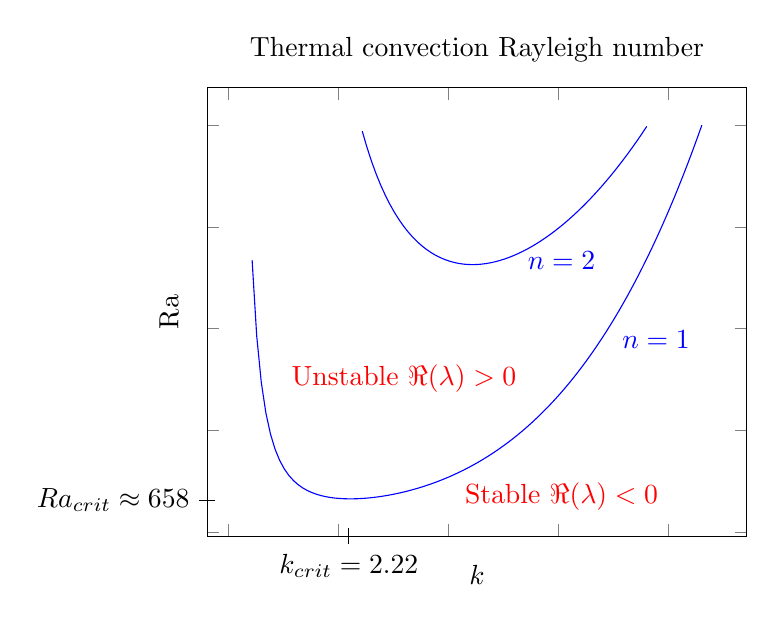
\begin{tikzpicture}
		\begin{axis}[title={Thermal convection Rayleigh
			number},ylabel={Ra},xlabel={$k$},yticklabels={,,},xticklabels={,,},
			samples=100,domain=0:10, restrict y to domain=0:8]
		%\draw[thick,->] (-0.1,0) -- (10, 0) node[right] {$k$};
		%\draw[thick,->] (0, -0.1) -- (0, 8) node[above] {Ra};
			\addplot[blue] plot[domain=0.353:8.611,samples=100] ({\x},{(pi^2 +
			\x^2)^3/(1000*\x^2)});
			\addplot[blue] plot[domain=0.353:8.611,samples=100] ({\x},{(4*pi^2 +
			\x^2)^3/(2000*\x^2)});
		\end{axis}
		\draw (0.1, 0.458) -- (-0.1, 0.458) node[left]
		{$\Ra_{\text{crit}} \approx 658$};
		\draw (1.8, 0.1) -- (1.8, -0.1) node[below] {$k_{\text{crit}} =
		2.22$};
		\draw[blue] (5.7, 2.5) node {$n=1$};
		\draw[blue] (4.5, 3.5) node {$n=2$};
		\draw[red] (4.5, 0.5) node {Stable $\Re(\lambda) < 0$};
		\draw[red] (2.5, 2) node {Unstable $\Re(\lambda) > 0$};
	\end{tikzpicture}
\end{center}

Results for other boundary conditions are:
\begin{itemize}
	\item Free--rigid boundary: $\Ra_{\text{crit}} \sim 1101, k_c = 2.68$
	\item Rigid--rigid boundary: $\Ra_{\text{crit}} \sim 1708, k_c = 3.117$
\end{itemize}

Notice that at criticality only the size of $k$ is specified, \emph{not} its
direction. Hence there are an infinite number of possibilities $\symbf{k} =
(k\cos\phi,k\sin\phi)$. Various different patterns which tesselate are as
follows.

\begin{enumerate}
	\item \textbf{2D rolls.} Orientate $x$-axis along $k$ such that $k_2 = 0$.
		We have velocity components ($w$ specified in problem, $u$ follows
		from incompressibility)
		\begin{align}
			w &= W(z) \sin kx \\
			v &= 0\\ 
			u &= \frac{\pi \cos \pi z \cos k x}{k}
		\end{align}

		\begin{center}
			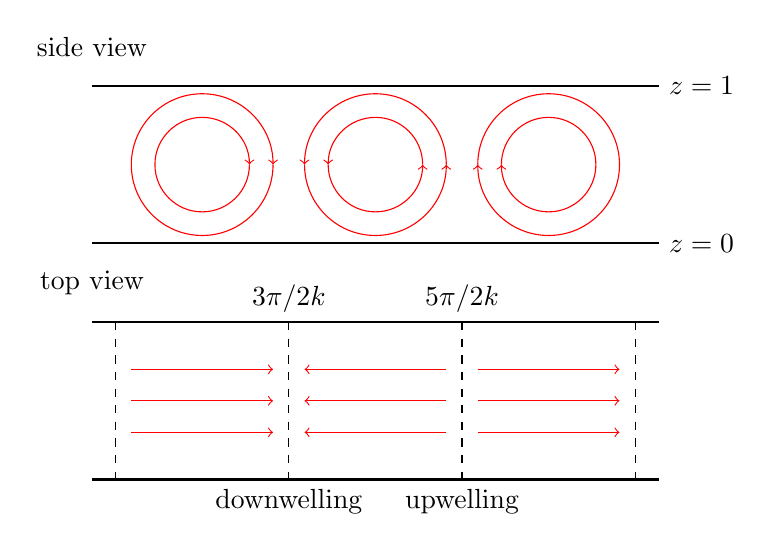
\begin{tikzpicture}
				\draw (0, 2.5) node {side view};
				\draw[thick] (0,0) -- (7.2, 0) node[right] {$z=0$};
				\draw[thick] (0,2) -- (7.2, 2) node[right] {$z=1$};
				\draw[red,<-] (2.3, 1) arc(0:360:0.9);
				\draw[red,<-] (2.0, 1) arc(0:360:0.6);
				\draw[red,->] (2.7, 1) arc(-180:0:0.9);
				\draw[red,->] (3.0, 1) arc(-180:0:0.6);
				\draw[red,->] (4.5, 1) arc(0:180:0.9);
				\draw[red,->] (4.2, 1) arc(0:180:0.6);
				\draw[red,<-] (4.9, 1) arc(-180:180:0.9);
				\draw[red,<-] (5.2, 1) arc(-180:180:0.6);
			\begin{scope}[shift={(0,-3)}]
				\draw (0, 2.5) node {top view};
				\draw[thick] (0,0) -- (7.2, 0);
				\draw[thick] (0,2) -- (7.2, 2);
				\draw[dashed] (2.5, 2) -- (2.5, 0) node[below] {downwelling};
				\draw[dashed] (4.7, 2) -- (4.7, 0) node[below] {upwelling};
				\draw[dashed] (6.9, 2) -- (6.9, 0);
				\draw[dashed] (0.3, 2) -- (0.3, 0);
				\draw (2.5, 2) node[above] {$3\pi/2k$};
				\draw (4.7, 2) node[above] {$5\pi/2k$};
				
				\draw[red,->] (0.5, 1.4) -- (2.3, 1.4);
				\draw[red,->] (0.5, 1) -- (2.3, 1);
				\draw[red,->] (0.5, 0.6) -- (2.3, 0.6);

				\draw[red,->] (4.5, 1.4) -- (2.7, 1.4);
				\draw[red,->] (4.5, 1) -- (2.7, 1);
				\draw[red,->] (4.5, 0.6) -- (2.7, 0.6);

				\draw[red,->] (4.9, 1.4) -- (6.7, 1.4);
				\draw[red,->] (4.9, 1) -- (6.7, 1);
				\draw[red,->] (4.9, 0.6) -- (6.7, 0.6);
			\end{scope}
			\end{tikzpicture}
		\end{center}
	\item \textbf{Rectangles.} Velocity components are
		\begin{align}
			w &= W(z) \cos k_1 x \cos k_2 y \\
			v &= -\frac{k_2}{k^2} W' \cos k_1 x \sin k_2 y \\
			u &= -\frac{k_1}{k^2} W' \sin k_1 x \cos k_2 y
		\end{align}
		\begin{center}
			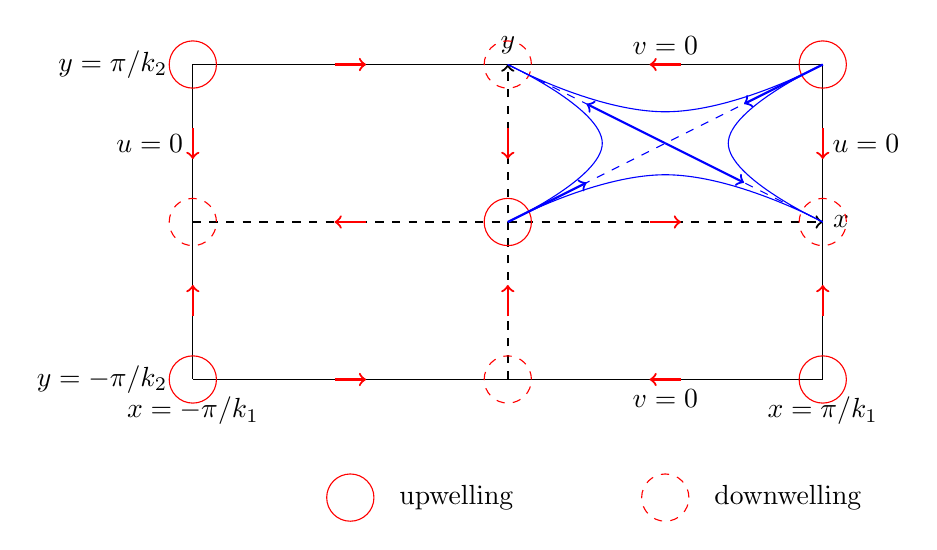
\begin{tikzpicture}
				\draw (0,0) -- (8,0) -- (8, 4) -- (0, 4) -- (0,0);
				\draw[dashed,thick,->] (4, 0) -- (4,4) node[above] {$y$};
				\draw[dashed,thick,->] (0, 2) -- (8,2) node[right] {$x$};

				\draw[blue,dashed] (4,2) -- (8, 4);
				\draw[blue,dashed] (4, 4) -- (8, 2);

				\draw[red,dashed] (0, 2) circle (0.3);
				\draw[red,dashed] (4, 0) circle (0.3);
				\draw[red,dashed] (4, 4) circle (0.3);
				\draw[red,dashed] (8, 2) circle (0.3);
				\draw[red] (0, 0) circle (0.3);
				\draw[red] (0, 4) circle (0.3);
				\draw[red] (8, 4) circle (0.3);
				\draw[red] (8, 0) circle (0.3);
				\draw[red] (4, 2) circle (0.3);

				\draw (0,-0.1) node[below] {$x=-\pi/k_1$};
				\draw (8,-0.1) node[below] {$x=\pi/k_1$};
				\draw (-0.2, 0) node[left] {$y=-\pi/k_2$};
				\draw (-0.2, 4) node[left] {$y=\pi/k_2$};

				\draw (6, 0) node[below] {$v=0$};
				\draw (6, 4) node[above] {$v=0$};
				\draw (0, 3) node[left] {$u=0$};
				\draw (8, 3) node[right] {$u=0$};

				\draw[red,thick,->] (6.2, 0) -- (5.8, 0);
				\draw[red,thick,->] (6.2, 4) -- (5.8, 4);
				\draw[red,thick,<-] (6.2, 2) -- (5.8, 2);
				\draw[red,thick,->] (1.8, 0) -- (2.2, 0);
				\draw[red,thick,->] (1.8, 4) -- (2.2, 4);
				\draw[red,thick,<-] (1.8, 2) -- (2.2, 2);
				\draw[red,thick,->] (0, 0.8) -- (0, 1.2);
				\draw[red,thick,->] (4, 0.8) -- (4, 1.2);
				\draw[red,thick,->] (8, 0.8) -- (8, 1.2);
				\draw[red,thick,<-] (0, 2.8) -- (0, 3.2);
				\draw[red,thick,<-] (4, 2.8) -- (4, 3.2);
				\draw[red,thick,<-] (8, 2.8) -- (8, 3.2);

				\draw[smooth,blue] plot[tension=0.8] coordinates {(4,2) (5.2, 3) (4, 4)};
				\draw[smooth,blue] plot[tension=0.8] coordinates {(8,2) (6.8, 3) (8, 4)};
				\draw[smooth,blue] plot[tension=0.8] coordinates {(4,4) (6, 3.4) (8, 4)};
				\draw[smooth,blue] plot[tension=0.8] coordinates {(4,2) (6, 2.6) (8, 2)};
				\draw[blue,thick,->] (4,2) -- (5, 2.5);
				\draw[blue,thick,->] (8,4) -- (7, 3.5);
				\draw[blue,thick,<-] (5,3.5) -- (6, 3);
				\draw[blue,thick,<-] (7,2.5) -- (6, 3);

				\draw[red] (2, -1.5) circle (0.3);
				\draw (2.5, -1.5) node[right] {upwelling};
				\draw[red,dashed] (6, -1.5) circle (0.3);
				\draw (6.5, -1.5) node[right] {downwelling};
			\end{tikzpicture}
		\end{center}
	\item \textbf{Hexagons.} Vertical velocity component
		\begin{equation}
			w = W(z) \left[ \cos \frac{k}{2}(\sqrt{3}x+y) + \cos \frac{k}{2}
			(\sqrt{3}x-y) + \cos ky \right]
		\end{equation}
		This is flow in a hexagon of side length $L = 4\pi/3k$.
		\begin{center}
			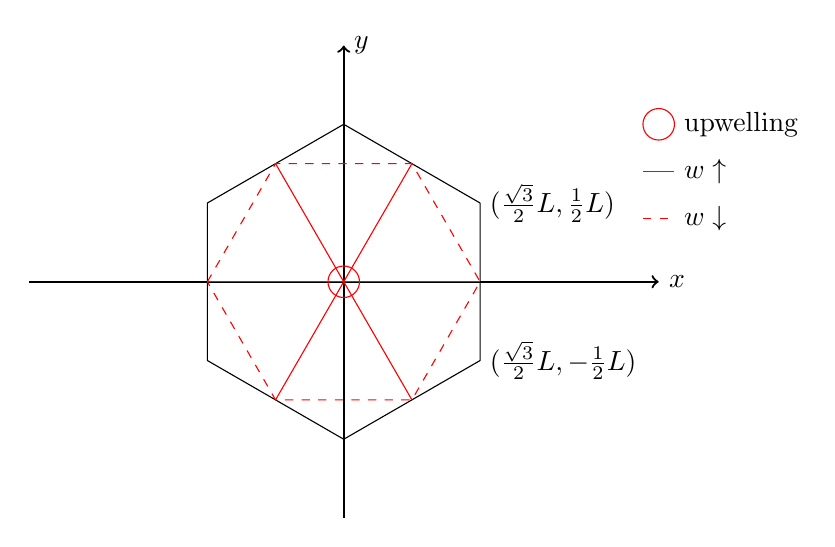
\begin{tikzpicture}[scale=2]
				\draw[thick,->] (-2, 0) -- (2,0) node[right] {$x$};
				\draw[thick,->] (0, -1.5) -- (0,1.5) node[right] {$y$};
				\draw[red] (0,0) circle (0.1);
				\draw (0.866, 0.5) -- (0, 1) -- (-0.866, 0.5) -- (-0.866,
				-0.5) -- (0, -1) -- (0.866, -0.5) -- (0.866, 0.5);
				\draw[red] (-0.433, -0.75) -- (0.433, 0.75);
				\draw[red] (0.433, -0.75) -- (-0.433, 0.75);
				\draw[red] (-0.866,0) -- (0.866, 0);

				\draw[red,dashed] (-0.866, 0) -- (-0.433, 0.75) -- (0.433,
				0.75) -- (0.866, 0) -- (0.433,-0.75) -- (-0.433, -0.75) --
				(-0.866,0);

				\draw (0.866, 0.5) node[right]
				{$(\frac{\sqrt{3}}{2}L,\frac{1}{2}L)$};
				\draw (0.866, -0.5) node[right]
				{$(\frac{\sqrt{3}}{2}L,-\frac{1}{2}L)$};

				\draw[red] (2, 1) circle (0.1);
				\draw (2.1, 1) node[right] {upwelling};
				\draw[red] (1.9, 0.7) -- (2.1, 0.7);
				\draw (2.1, 0.7) node[right] {$w \uparrow$};
				\draw[red,dashed] (1.9, 0.4) -- (2.1, 0.4);
				\draw (2.1, 0.4) node[right] {$w \downarrow$};
			\end{tikzpicture}
		\end{center}
\end{enumerate}

\section{Centrifugal instabilities}
Flows with curved streamlines can be unstable due to centrifugal effects.
\subsection{Rayleigh's criterion}
We will concentrate on axisymmetric flows. Consider an azimuthal flow 
\begin{equation}
	\u = u_\theta(r)\hat{\symbf{\theta}} = r \Omega(r)\hat{\symbf{\theta}}
\end{equation}
The inviscid, axisymmetric equations for a general flow $\u = u_r
\hat{\symbf{r}} + u_\theta \hat{\symbf{\theta}} + u_z \hat{\symbf{z}}$ are

\begin{align}
	\frac{\partial u_r}{\partial t} + \u \cdot \nabla u_r -
	\frac{u_\theta^2}{r} &= - \frac{1}{\rho}\frac{\partial p}{\partial r} \\
	\frac{\partial u_\theta}{\partial t} + \u \cdot \nabla u_\theta +
	\frac{u_r u_\theta}{r} &= - \cancel{\frac{1}{\rho}\frac{1}{r}\frac{\partial
p}{\partial \theta}} \\
	\frac{\partial u_z}{\partial t} + \u \cdot \nabla u_z
	 &= - \frac{1}{\rho}\frac{\partial p}{\partial z} \\
	 \frac{1}{r}\frac{\partial}{\partial r}(ru_r) +
	 \cancel{\frac{1}{r}\frac{\partial u_\theta}{\partial \theta}} +
			\frac{\partial u_z}{\partial z} &= 0 
\end{align}
where $\u \cdot \nabla = u_r \frac{\partial}{\partial r} + \cancel{
\frac{u_\theta}{r}\frac{\partial}{\partial \theta}} + u_z
\frac{\partial}{\partial z}$. Cancelled terms are absent in the axisymmetric
setting. The \emph{centrifugal} term is $-u_\theta^2/r$ in the $r$-momentum
equation. The $\theta$-momentum equation can be rearranged, and multiplied by
$r$ to give a material conservation equation:
\begin{align}
	\frac{\partial}{\partial r} (ru_\theta) + r u_r \frac{\partial
	u_\theta}{\partial r} + u_z \frac{\partial}{\partial z} (ru_\theta) +
	r\left(\frac{u_r u_\theta}{r}\right) &= 0 \\
	\implies \frac{\partial}{\partial t} (ru_\theta) + u_r
	\frac{\partial}{\partial r}(ru_\theta) + u_z \frac{\partial}{\partial
z}(ru_\theta) &= 0  \\
\implies \frac{\diffD}{\diffD t} (ru_\theta) &= 0
\end{align}

This expresses conservation of angular momentum: the angular momentum per unit
mass is $I = ru_\theta$, hence $\frac{\diffD I}{\diffD t} = 0$. This result
also follows from Kelvin's circulation theorem, using the circulation $\Gamma
= 2\pi r u_\theta$ for an inviscid fluid. The statement says that if $\u =
u_\theta(r)\hat{\symbf{\theta}}$ (i.e. axisymmetric azimuthal flow) then $I =
I(r)$ is a basic state.


\paragraph{What distributions of $I(r)$ could be stable?}
Rayleigh's argument considers 2 rings of fluid at radius $r_1$ and $r_2 (>
r_1)$ respectively. 
\begin{center}
	\begin{tikzpicture}
		\draw[thick,blue,->] (0,0) [partial ellipse=0:360:2 and .7];
		\draw[thick,blue,->] (0,0) [partial ellipse=0:360:2.5 and .9];
		\draw (0,0)  -- (2, 0) node[midway,below] {$r_1$};
		\draw (0,0)  -- (1.5, 0.72) node[midway,above] {$r_2$};
		\draw[thick,->] (0,0) -- (0, 1.5);
	\end{tikzpicture}
\end{center}

The kinetic energy is
\begin{equation}
	E = \frac{1}{2}\rho\left(\frac{I_1^2}{r_1^2} + \frac{I_2^2}{r_2^2}\right)
\end{equation}
Now suppose the rings swap places due to a perturbation, but they keep their
angular momentum (since it is materially conserved). The new KE is
\begin{equation}
	E_{\text{new}} = \frac{1}{2} \left( 
	\frac{I_2^2}{r_1^2} + \frac{I_1^2}{r_2^2}\right)
\end{equation}
Hence the swap has resulted in an energy change
\begin{equation}
	\Delta E = (I_2^2-I_1^2)\left(\frac{1}{r_1^2} - \frac{1}{r_2^2}\right)
\end{equation}
We can expect instability if $\Delta E < 0$. Since $r_2 > r_1$, the second
factor is positive hence
\begin{equation}
	\Delta E < 0 \iff I_2^2 < I_1^2
\end{equation}
Hence Rayleigh's criterion for stability is $I_2^2 \ge I_1^2$ or equivalently
\begin{equation}
	\frac{\diffd I^2}{\diffd r} \ge 0
\end{equation}
i.e. angular momentum does not increase outwards. Note that with $I =
ru_\theta = r^2 \Omega$ we have the condition
\begin{equation}
	\frac{\diffd}{\diffd r}\left( r^4 \Omega^2 \right) \ge 0
\end{equation}
for stability. This is often written using the \emph{Rayleigh determinant}
\begin{equation}
	\Phi \equiv \frac{1}{r}
	\frac{\diffd}{\diffd r}\left( r^4 \Omega^2 \right)
\end{equation}
Hence stability is predicted if $\Phi \ge 0$.

\subsection{Derivation via linear stability analysis}
Consider Taylor-Couette geometry: cylindrical walls at $r_1$ and $r_2$ with an
inviscid base state $\u = r \Omega(r) \hat{\symbf{\theta}}$, with axisymmetric
perturbations $\u'$. We have incompressibility
\begin{equation}
	\nabla \cdot \u' = 0 \implies \frac{1}{r}\frac{\partial}{\partial
	r}(ru_r') + \frac{\partial u_z'}{\partial z} = 0
\end{equation}
The Euler equations for this perturbation are
\begin{align}
	\frac{\partial u_r'}{\partial t} - \frac{2r \Omega u_\theta'}{r} &=
	-\frac{1}{\rho} \frac{\partial p'}{\partial r} \\
	\frac{\partial u_\theta'}{\partial t} + u_r'\frac{\diffd}{\diffd
r}(r\Omega) + \frac{u_r' r \Omega}{r} &= 0 \\
\frac{\partial u_z'}{\partial t} &= -\frac{1}{\rho}\frac{\partial p'}{\partial
z}
\end{align}
Now specify normal mode decomposition
\begin{equation}
	\begin{pmatrix} u_r' \\ u_\theta' \\ u_z' \\ p' \end{pmatrix} = 
	\begin{pmatrix} \hat{u}_r(r) \\ \hat{u}_\theta(r) \\ \hat{u}_z(r) \\
	\hat{p}(r) \end{pmatrix} e^{ikz + \sigma t}
\end{equation}
Only axisymmetric perturbations are considered. The Euler equations become
\begin{align}
	\frac{1}{r}\frac{\diffd}{\diffd r}(r\hat{u}_r) + ik \hat{u}_z &= 0 \\
	\sigma \hat{u}_r - 2\Omega \hat{u}_\theta &= - \frac{1}{\rho} \frac{\diffd
	\hat{p}}{\diffd r} \\
		\sigma \hat{u}_\theta + \hat{u}_r(\Omega + (r\Omega)_r) &= 0 \\
		\sigma \hat{u}_z &= -\frac{1}{\rho} ik \hat{p}
\end{align}
We can reduce this system down to a single equation for $\hat{u}_r$:
\begin{equation}
	\frac{\diffd}{\diffd r}\left(\frac{\diffd}{\diffd r} +
	\frac{1}{r}\right)\hat{u}_r - k^2 \hat{u}_r -2\frac{k^2}{\sigma^2}
	\Omega(2\Omega + r\Omega')\hat{u}_r = 0
\end{equation}
This is a second order ODE for $\hat{u}_r$ with BCs $\hat{u}_r = 0$ at $r=
r_1, r_2$. For this flow, Rayleigh's determinant is
\begin{equation}
	\Phi \equiv \frac{1}{r}
	\frac{\diffd}{\diffd r}\left( r^4 \Omega^2 \right) = 4\Omega^2 + 2r\Omega'
	\Omega
\end{equation}
Hence the ODE for $\hat{u}_r$ may be written as
\begin{equation}
	\frac{\diffd}{\diffd r}\left(\frac{1}{r}\frac{\diffd}{\diffd
	r}(r\hat{u}_r)\right) - k^2 \hat{u}_r = \frac{k^2}{\sigma^2} \Phi(r)
	\hat{u}_r
	\label{eq:l5}
\end{equation}
Multiply \eqref{eq:l5} by $r\hat{u}_r^*$ (complex conjugate) and integrate
from $r_1$ to $r_2$:
\begin{equation}
	\int_{r_1}^{r_2} r \hat{u}_r^* \frac{\diffd}{\diffd r} \left(
	\frac{1}{r}\frac{\diffd}{\diffd r}(r\hat{u}_r)\right) \diffd r - k^2
	\int_{r_1}^{r_2} r \abs{\hat{u}_r}^2 \, \diffd r = \frac{k^2}{\sigma^2}
	\int_{r_1}^{r_2} r \Phi \abs{\hat{u}_r}^2 \, \diffd r
\end{equation}
The first term may be integrated by parts to give:
\begin{equation}
	\cancel{\left[ r\hat{u}_r^* \frac{1}{r} \frac{\diffd}{\diffd
	r}(r\hat{u}_r)\right]_{r_1}^{r_2}}
	-\int_{r_1}^{r_2} \frac{\diffd}{\diffd r}(r \hat{u}_r^*)\frac{1}{r} \frac{\diffd}{\diffd r} (r\hat{u}_r) \diffd r - k^2
	\int_{r_1}^{r_2} r \abs{\hat{u}_r}^2 \, \diffd r = \frac{k^2}{\sigma^2}
	\int_{r_1}^{r_2} r \Phi \abs{\hat{u}_r}^2 \, \diffd r
\end{equation}
The first term vanishes since $\hat{u}_r =0$ at $r=r_1,r_2$. Labelling the
first integral as $H_1 > 0$ and the second as $H_2 > 0$, we have
\begin{equation}
	\frac{k^2}{\sigma^2}
	\int_{r_1}^{r_2} r \Phi \abs{\hat{u}_r}^2 \, \diffd r = -H_1 - k^2 H_2 < 0
\end{equation}
If $\Phi \ge 0$ then $\sigma^2 < 0$, i.e. $\sigma$ is imaginary and we have
stability. If instead $\Phi < 0$ somewhere in the domain, then potentially
\begin{equation}
	\int_{r_1}^{r_2} r \Phi \abs{\hat{u}_r}^2 \, \diffd r < 0
\end{equation}
in which case $\sigma^2 > 0$ and we have instability. Hence $\Phi < 0$
somewhere in the domain is \emph{necessary} (but not sufficient) condition for
instability. So this formal analysis confirms Rayleigh's heuristic criterion.
Note, really we need to consider non-axisymmetric perturbations too.

\subsection{Taylor vortices}
Apply Rayleigh's criterion to Taylor-Couette flow.
\begin{center}
	\begin{tikzpicture}
		\draw[thick,name path =A] (0,0) ellipse (1 and 0.2);
		\draw[thick,name path =B] (0,0) ellipse (1.5 and 0.4);
		\draw (0,-3) ellipse (1 and 0.2);
		\draw[thick] (0,-3) [partial ellipse = -180:0:1.5 and 0.4];
		\draw (0,-3) [partial ellipse = 0:180:1.5 and 0.4];
		\draw[->] (0,0) [partial ellipse = -10:60:1.6 and 0.5]
		node[midway,above] {$\Omega_2$};
		\draw[->] (0,0) [partial ellipse = -10:50:0.9 and 0.15]
		node[midway,left] {$\Omega_1$};
		\draw[thick] (1.5,0) -- (1.5, -3);
		\draw[thick] (-1.5, 0) -- (-1.5, -3);
		\draw (1, 0) -- (1, -3);
		\draw (-1, 0) -- (-1, -3);
		\draw[dashed] (0,1) -- (0, -3);
		\draw[<->] (0,-1.2) -- (1, -1.2) node[midway,above] {$R_1$};
		\draw[<->] (0,-2) -- (1.5, -2) node[midway,above] {$R_2$};
		\tikzfillbetween[of=A and B]{blue, opacity=0.2}
	\end{tikzpicture}
\end{center}

When viscosity is present, the general solution with $\partial_\theta =
\partial_z = 0$ is
\begin{equation}
	u_\theta(r) = A r + \frac{B}{r}
\end{equation}
No-slip boundary conditions at $r=R_1,R_2$ give
\begin{equation}
	A = \frac{\Omega_2 R_2^2 - \Omega_1 R_1^2}{R_2^2 - R_1^2}, \hspace{2em} B
	= \frac{\Omega_1 - \Omega_2}{R_1^{-2} - R_2^{-2}}
\end{equation}
Note this solves $(\nabla^2 - 1/r^2)u_\theta = 0$ where $\nabla^2 =
\frac{1}{r}\partial_r(r \partial_r)$. In this case $\Omega = u_\theta/r = A +
B/r^2$ hence Rayleigh's determinant is
\begin{equation}
	\Phi = \frac{1}{r^3} \frac{\diffd}{\diffd r}\left(r^4 \Omega^2\right) =
	\frac{1}{r^3} \frac{\diffd}{\diffd r} \left[ r^4 \left(A^2 + \frac{2AB}{r^2} +
	\frac{B^2}{r^4}\right)\right] = 4A^2\left(1+\frac{B}{Ar^2}\right)
\end{equation}
For convenience we define $\mu = \Omega_2/\Omega_1$ and $\eta = R_1 / R_2 <
1$. Then
\begin{equation}
	\Phi = 4A^2 \left[ 1 - \frac{(1-\mu)R_1^2}{(\eta^2 - \mu)r^2}\right]
\end{equation}
For stability, i.e. $\Phi \ge 0$ everywhere, we require for all $r \in \left[
R_1, R_2\right]$
\begin{equation}
	1 \ge \frac{(1-\mu)R_1^2}{(\eta^2 - \mu)r^2} \ge \frac{1-\mu}{\eta^2 -
	\mu}
\end{equation}
where the last inequality follows since $R_1^2 / r^2 \ge 1$ for all $r \in
\left[R_1, R_2\right]$. 
There are now two cases: 
\begin{itemize}
	\item If $\eta^2 > \mu$ then
	\begin{equation}
		\eta^2 - \mu \ge 1-\mu \implies \eta^2 \ge 1 
	\end{equation}
	This is a contradiction since $\eta < 1$. 
	\item Otherwise $\eta^2 < \mu$, so
	\begin{equation}
		\eta^2 - \mu \le 1 - \mu \implies \eta^2 \le 1
	\end{equation}
\end{itemize}
Thus Rayleigh's criterion is $\eta^2 < \mu$ for stability.

\begin{center}
	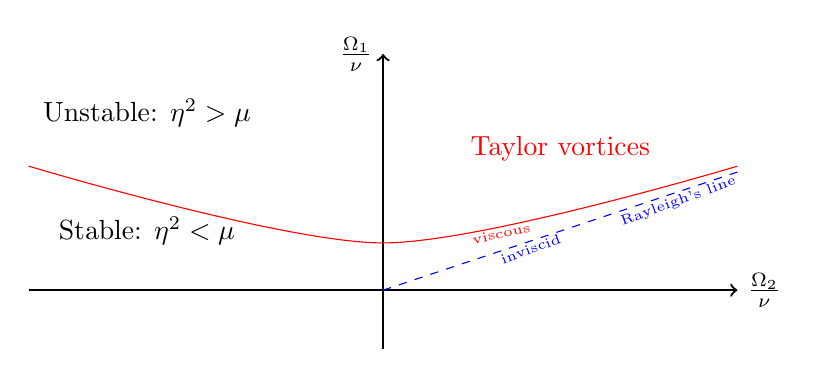
\begin{tikzpicture}[scale=1.5]
		\draw[thick,->] (-3,  0) --  (3, 0) node[right]
		{$\frac{\Omega_2}{\nu}$};
		\draw[thick,->] (0,  -0.5) --  (0, 2) node[left]
		{$\frac{\Omega_1}{\nu}$};
		\draw[dashed,blue] (0,0) -- (3, 1);
		\draw[red] plot[smooth] coordinates {(-3, 1.05) (0, 0.4) (3, 1.05)};
		\draw[red] (1, 0.48) node[rotate=12]{\tiny viscous};
		\draw[blue] (1.25, 0.35) node[rotate=20] {\tiny inviscid};
		\draw[blue] (2.5, 0.75) node[rotate=20] {\tiny Rayleigh's line};
		\draw (-2, 0.5) node {Stable: $\eta^2 < \mu$};
		\draw (-2, 1.5) node {Unstable: $\eta^2 > \mu$};
		\draw[red] (1.5, 1.2) node {Taylor vortices};
	\end{tikzpicture}
\end{center}

For a fixed geometry (i.e. fixed $\eta$) we can plot a stability diagram, with
Rayleigh's line $\eta^2 = \mu = \Omega_2 / \Omega_1$ marking the stability
heuristic. In Taylor-Couette geometry, the instability often manifests itself
as \emph{Taylor vortices}, though there are many different modes of
instability depending on $\Omega_1, \Omega_2, \nu$.

\begin{figure}
	\centering
	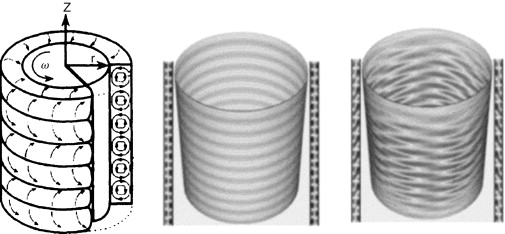
\includegraphics[width=0.5\textwidth]{taylor_vortices.jpg}
	\caption{Taylor vortices, from Dutta and Ray, 2004.}
\end{figure}

\section{Parallel shear flows}
For some flows, inviscid analysis gives a good approximation to the stability
properties of a viscous fluid (e.g. Kelvin-Helmholtz, Taylor-Couette flow) but
for others, it does not (e.g. plane Couette flow, channel flow, pipe  flow).
In these flows, viscosity can be \emph{de}stabilising.

\begin{center}
	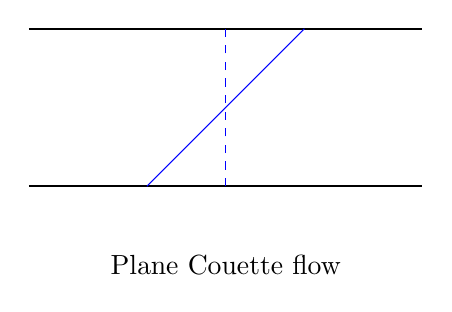
\begin{tikzpicture}
		\draw[thick] (0,0) -- (5, 0);
		\draw[thick] (0, 2) -- (5, 2);
		\draw[blue,dashed]  (2.5,0) -- (2.5, 2);
		\draw[blue] (1.5,0) -- (3.5, 2);
		\draw (2.5, -1) node {Plane Couette flow};
	\end{tikzpicture}
	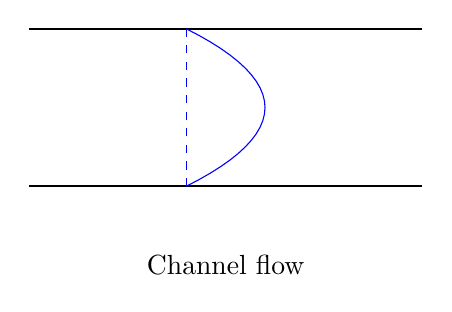
\begin{tikzpicture}
		\draw[thick] (0,0) -- (5, 0);
		\draw[thick] (0, 2) -- (5, 2);
		\draw[blue,dashed]  (2,0) -- (2, 2);
		\draw[blue] plot[domain=1:-1] ({3-\x*\x},{1+\x});
		\draw (2.5, -1) node {Channel flow};
	\end{tikzpicture}
	\begin{tikzpicture}
		\draw[thick] (1,0) -- (4, 0);
		\draw[thick] (1, 2) -- (4, 2);
		\draw[thick] (1, 1) [partial ellipse = -90:-270:0.5 and 1];
		\draw[thick] (4, 1) ellipse (0.5 and 1);
		\draw[blue,dashed]  (2,0) -- (2, 2);
		\draw[blue] plot[domain=1:-1] ({3-\x*\x},{1+\x});
		\draw (2.5, -1) node {Pipe flow};
	\end{tikzpicture}
\end{center}

\subsection{Inviscid analysis}
Consider a parallel shear flow $U(z)\hat{\symbf{x}}$. The non-dimensionalised
Euler equations are
\begin{align}
	\frac{\partial \u}{\partial t} + \u \cdot  \nabla \u &= - \nabla p \\
	\nabla \cdot \u &= 0
\end{align}
with boundary conditions $\u \cdot \hat{\symbf{z}} = 0$ at $z=z_1,z_2$. The
basic flow is $\symbf{U} = U(z)\hat{\symbf{x}}$ with $P$ constant -- any
constant form of the pressure is valid.  Add small perturbations
\begin{equation}
	\u = U(z)\hat{\symbf{x}} + \u', \hspace{1em}p = P + p'
\end{equation}
The Euler equations become
\begin{align}
	\frac{\partial \u'}{\partial t} + U\frac{\partial \u'}{\partial x} + w'
	\frac{\diffd U}{\diffd z} \hat{\symbf{x}} &= - \nabla p' \\
	\nabla \cdot \u' &= 0 
\end{align}
with boundary conditions $w' = 0$ at $z=z_1, z_2$. All equations have
coefficients independent of $x, y, t$ so we can separate the variables by
taking normal modes of the form
\begin{align}
	\u'(\x,t) &= \hat{\u}(z) e^{i(\alpha x  + \beta y - \alpha c t)} \\
	p'(\x,t)  &= \hat{p}(z) e^{i(\alpha x+ \beta y - \alpha c t)}
\end{align}
Note we have replaced the usual $\sigma$ with $-i\alpha c$. It is understood
that the physical fluid perturbation velocity $\u'$ is represented by the real
part, e.g.
\begin{equation}
	w' = \left[ \Re(\hat{w})\cos(\alpha x + \beta y - \alpha c_r t)
	-\Im(\hat{w})\sin(\alpha x+\beta y - \alpha c_r t)\right] e^{\alpha c_i t}
\end{equation}
This mode is a wave travelling with phase speed  $\alpha c_r /\sqrt{\alpha^2 +
\beta^2}$ in the $(\alpha, \beta, 0)$ direction and it decays like $e^{\alpha
c_i t}$ for $c_i < 0$, or grows if $c_i > 0$.  The equations are now
\begin{align}
i\alpha (U-c)\hat{u} + \frac{\diffd U}{\diffd z} \hat{w} + i \alpha\hat{p} &=
0 \label{eq:l6:1}\\
i\alpha (U-c)\hat{v} +  i \beta\hat{p} &=
0 \label{eq:l6:2} \\
i\alpha (U-c)\hat{w} +  \frac{\diffd \hat{p}}{\diffd z} &=
0 \label{eq:l6:3}\\
i\alpha \hat{u} + i\beta \hat{v} + \frac{\diffd \hat{w}}{\diffd z} &=
0\label{eq:l6:4}
\end{align}
with boundary conditions  $\hat{w}= 0$ at $z=z_1, z_2$. This is an eigenvalue
problem in $c \in \mathbb{C}$. Instability  corresponds to $c_i > 0$ and $c_i
\le 0$ for stability.

\subsubsection{Squire's transformation (Squire, 1933)}
Before  attempting to solve \eqref{eq:l6:1}--\eqref{eq:l6:4}, we consider
Squire's transformation. Define the transformed variables
\begin{equation}
	\tilde{\alpha} = \sqrt{\alpha^2 + \beta^2},\hspace{1em} \tilde{u} =
	\frac{\alpha \hat{u} + \beta \hat{v}}{\tilde{\alpha}}, \hspace{1em}
	\tilde{p} = \frac{\tilde{\alpha}\hat{p}}{\alpha}
\end{equation}
Construct $(\alpha\eqref{eq:l6:1} + \beta\eqref{eq:l6:2})/\alpha$:
\begin{equation}
	i\tilde{\alpha}(U-c)\tilde{u} + \frac{\diffd  U}{\diffd z} \hat{w} +
	i\tilde{\alpha}\tilde{p} =  0\label{eq:l6:5}
\end{equation}
Similarly $\tilde{\alpha}\eqref{eq:l6:3}/\alpha$:
\begin{equation}
	i\tilde{\alpha}(U-c)\hat{w} + \frac{\diffd \tilde{p}}{\diffd z} =
	0\label{eq:l6:6}
\end{equation}
Incompressibility is now expressed as
\begin{equation}
	i\tilde{\alpha}\tilde{u}  + \frac{\diffd \hat{w}}{\diffd z} = 0
\end{equation}

The transformed system has the same form as \eqref{eq:l6:1}--\eqref{eq:l6:4}
with $\beta = \hat{v} = 0$ and $\alpha \to \tilde{\alpha},
\hat{u}\to\tilde{u}, \hat{p}\to\tilde{p}$ but $c$ unchanged. Thus the
eigenvalue $c$ depends on $\sqrt{\alpha^2+\beta^2}$ but the growth rate is
$\alpha c_i$. So the largest growth rate $\alpha c_i$ is given by $\beta = 0$
for all wavenumber pairs $(\alpha,\beta)$ with $\sqrt{\alpha^2 + \beta^2}$
constant. Hence it is sufficient to consider $\beta = 0$ disturbances only. To
any unstable 3D mode $\alpha \ne 0, \beta \ne 0$ there corresponds a more
unstable 2D mode with $\beta = 0$.

\subsubsection{Rayleigh's equation}
Work in 2D (Squires). Use streamfunction $\psi'$ such that
\begin{equation}
	u' = \psi_z', \,\,v' = 0, \,\,w' = -\psi_x'
\end{equation}
Further, let $\psi'(x,z,t) = \phi(z)e^{i\alpha(x-ct)}$ so that it is  now
clear that $c_r$ is the phase speed in the $x$ direction. Now $\hat{u} =
\frac{\diffd \phi}{\diffd z}$ and $\hat{w} = -i\alpha \phi$ (notice the phase
difference). Then \eqref{eq:l6:5} becomes
\begin{align}
	i\alpha(U-c)\frac{\diffd \phi}{\diffd z} + \frac{\diffd U}{\diffd
	z}(-i\alpha \phi) + i\alpha \hat{p} &= 0\\
	\implies \hat{p}&= \frac{\diffd U}{\diffd z}\phi - (U-c)\frac{\diffd
	\phi}{\diffd z}
\end{align}
Substituting into \eqref{eq:l6:6} gives
\begin{align}
	i\alpha (U-c)(-i\alpha \phi) + \frac{\diffd}{\diffd z}\left[ \frac{\diffd
	U}{\diffd z}\phi - (U-c)\frac{\diffd \phi}{\diffd z}\right] &= 0 \\
	\implies (U-c)(\phi'' - \alpha^2 \phi) - U'' \phi &=0
\end{align}
with boundary conditions $\phi = 0$ at $z=z_1, z_2$. This is \emph{Rayleigh's
equation (1880)}.
\paragraph{Comments.}
\begin{itemize}
	\item Rayleigh's equation involves $\alpha^2$ only so need only consider
		$\alpha > 0$.
	\item If $(\phi,c)$ solves the problem then so does $(\phi^*, c^*)$. So if
		there exists a growing mode, there  also exists a corresponding
		decaying mode. Hence stability means $c \in \mathbb{R}$ for all
		$\alpha$.
	\item A singularity  exists at $U(z_c) = c$ -- this is called a critical
		layer and only occurs when $c \in \mathbb{R}$. Critical layers are
		important in solving IVPs and relating Rayleigh's equation to its
		viscous analogue, the Orr-Sommerfield equation (see later).
	\item There are two types of eigensolution:
		\begin{itemize}
			\item Continuous  spectrum $c \in \left[ \min U, \max
				U\right]$ and $\phi$ has a discontinuous derivative at $z_c$.
				This type of solution is never unstable.
			\item Discrete spectrum of complex conjugate pairs. This solution
				can be unstable.
		\end{itemize}
\end{itemize}

\subsubsection{Properties of Rayleigh's equation.}
\paragraph{Inflection point criterion.}
Suppose $c_i > 0$, i.e. consider an unstable mode. Multiply Rayleigh's
equation by $\phi^*$ and integrate from $z_1$ to $z_2$:
\begin{equation}
	\int_{z_1}^{z_2} \left[\phi^* \phi'' - \alpha^2 \abs{\phi}^2 - \frac{U''}{U-c}
	\abs{\phi}^2 \right]\diffd z = 0
\end{equation}
Integrate the first term by parts and note $\phi = \phi^* = 0$ at $z_1$ and
$z_2$. Hence
\begin{equation}
	\int_{z_1}^{z_2} \left[\abs{\phi'}^2  + \alpha^2 \abs{\phi}^2 +
	\frac{U''}{U-c}\abs{\phi}^2 \right] \diffd z =0
\end{equation}
Take imaginary part:
\begin{align}
	\Im \left[ \int_{z_1}^{z_2} \frac{U''(U-c^*)}{\abs{U-c}^2} \abs{\phi}^2
	 \diffd z \right]&= 0 \\
\implies
	-c_i\int_{z_1}^{z_2} \frac{U''}{\abs{U-c}^2} \abs{\phi}^2
	\diffd z &= 0
\end{align}
But $c_i > 0$ so we must have
\begin{equation}
\int_{z_1}^{z_2} \frac{U''}{\abs{U-c}^2} \abs{\phi}^2
	\diffd z  = 0
\end{equation}
Now $\abs{U-c}^2 > 0$ and $\abs{\phi}^2 > 0 $ so $U''$ must change sign
somewhere in $\left[z_1,z_2\right]$. Thus $U''=0$ at least once is a necessary
condition for inviscid instability, called the \emph{inflection point
criterion}.
\end{document}
